\documentclass[11pt]{article}

\usepackage[margin=1in]{geometry}
\usepackage{amsmath,amssymb}
\usepackage{graphicx}
\usepackage{booktabs}
\usepackage{hyperref}
\usepackage{natbib}
\usepackage{xcolor}

\title{\textbf{QAT-VQ: A Corrected Hybrid of Quantization-Aware Training and\\
Vector Quantization for Transformer Compression}}

\author{
  Md Abdur Rahman \\
  Department of Electrical \& Computer Engineering \\
  Rajshahi University of Engineering \& Technology (RUET) \\
  \texttt{abdurrahmanrussel77@gmail.com}
}

\date{}

\begin{document}
\maketitle

\begin{abstract}
Combining quantization-aware training (QAT) with vector quantization (VQ) is
an intuitively appealing way to compress transformer language models: QAT
preserves accuracy under low-precision constraints, while VQ exploits weight
redundancy beyond what scalar quantization can reach. In practice, however,
a naively combined QAT+VQ pipeline can perform \emph{worse} than either
technique alone if the vector codebook is too coarse or is applied to the
wrong tensors. We present a corrected QAT-VQ design --- product
quantization on feed-forward weights with a properly sized codebook,
combined with per-channel INT8 quantization on attention weights and
embeddings --- and evaluate it against post-training quantization (PTQ),
QAT alone, and two literature-standard post-training baselines, GPTQ
\citep{frantar2023gptq} and AWQ \citep{lin2024awq}, implemented from
scratch. On DistilBERT/SST-2, our hybrid achieves the best accuracy
(91.28\%, versus 91.06\% baseline) at the smallest size (53.7~MB, a
4.99$\times$ compression), beating every baseline including GPTQ and AWQ
on both axes simultaneously. On GPT-2/WikiText-2, the hybrid does not beat
PTQ outright but forms a genuine Pareto point, 23\% smaller for a
$\sim$1\% perplexity cost. A scaling study across GPT-2 at 124M, 355M, and
774M parameters (all on matched WikiText-103 calibration data) shows that
the compression ratio improves monotonically with scale (5.14$\times$
$\rightarrow$ 5.55$\times$ $\rightarrow$ 5.73$\times$), while the
perplexity gap versus PTQ does \emph{not} shrink monotonically
(+1.68\% $\rightarrow$ +1.30\% $\rightarrow$ +2.59\%) --- a nuanced,
non-monotonic finding we report honestly rather than force-fitting to a
simpler two-point narrative. We also observe that a simple INT8-only
baseline flips from outperforming the uncompressed model at small scale to
underperforming it by 4.1\% at 774M parameters, suggesting scale-dependent
quantization sensitivity is not unique to vector quantization. Code,
trained checkpoints, and full experiment logs are publicly available.
\end{abstract}

\section{Introduction}

Deploying large language models on resource-constrained hardware requires
reducing their memory footprint without unacceptable accuracy loss. Three
families of techniques dominate: post-training quantization (PTQ), which
applies quantization after training with no gradient updates
\citep{dettmers2022bit8}; quantization-aware training (QAT), which
simulates low-precision arithmetic during training so the model adapts to
it \citep{zafrir2019q8bert}; and vector quantization (VQ), which clusters
weight vectors into a shared codebook rather than quantizing each scalar
independently \citep{gong2014compressing}. Each has complementary
strengths: PTQ is cheap and fast, QAT preserves more accuracy at the cost
of retraining, and VQ can compress further than uniform scalar
quantization by exploiting correlations between weight elements.

Combining QAT and VQ is a natural idea, but a naive combination can fail.
In particular, we find that (1) an undersized codebook destroys weight
information beyond what any amount of fine-tuning can recover, and (2)
applying vector quantization to \emph{activations} rather than
\emph{weights} compounds error at every layer of the forward pass. Both
pitfalls can cause a hybrid method to underperform even the simplest PTQ
baseline. This paper presents a corrected design that avoids both, and
evaluates it rigorously: against internal ablations (PTQ, QAT alone),
against literature-standard baselines (GPTQ, AWQ) implemented independently
rather than assumed, across two task types (classification and
generation), and across three model scales spanning a 6$\times$ parameter
range.

\paragraph{Contributions.}
\begin{itemize}
  \item A corrected QAT-VQ design: 4-bit product quantization on
    feed-forward weights (the bulk and most redundant portion of a
    transformer), INT8 on attention weights and embeddings, with an
    optional codebook fine-tuning step.
  \item Evaluation against GPTQ and AWQ, implemented from scratch and
    verified against synthetic layers with structured activation
    correlation, showing our hybrid is competitive with or superior to
    these established methods, not just to weak internal baselines.
  \item A controlled scaling study (124M / 355M / 774M parameters, matched
    data) showing compression improves monotonically with scale while the
    quality-vs-compression trade-off does not --- including the process of
    diagnosing and resolving a real data-calibration confound between
    scale points, reported as part of the methodology.
  \item A qualitative check of generated text (not just perplexity),
    showing the primary visible artifact of compression is a mild
    increase in repetition, not incoherence.
\end{itemize}

\section{Related Work}

\textbf{Post-training and quantization-aware methods.} Q8BERT
\citep{zafrir2019q8bert} showed INT8 QAT preserves BERT accuracy on
downstream tasks. LLM.int8() \citep{dettmers2022bit8} demonstrated
mixed-precision decomposition for PTQ at scale. GPTQ
\citep{frantar2023gptq} introduced Hessian-guided, error-compensated
sequential quantization that substantially outperforms naive
round-to-nearest PTQ at the same bit-width, particularly at 3--4 bits on
large models. AWQ \citep{lin2024awq} instead identifies and protects
salient weight channels via activation-aware per-channel scaling prior to
quantization, avoiding GPTQ's more expensive per-layer calibration.

\textbf{Vector quantization for compression.} \citet{gong2014compressing}
applied product quantization to compress convolutional network weights,
establishing that clustering correlated weight sub-vectors captures more
redundancy than independent scalar quantization. Prior work combining VQ
with transformer-scale language models specifically, alongside
training-time quantization awareness, remains comparatively sparse --- the
gap this work addresses.

\textbf{Distillation and smaller base models.} DistilBERT
\citep{sanh2019distilbert} and GPT-2 \citep{radford2019gpt2} are the two
model families used throughout this work; distillation is complementary to
(not a substitute for) post-hoc compression, and both techniques are
commonly applied together in deployment settings.

\section{Method}

\subsection{Product Quantization on Feed-Forward Weights}

For a weight matrix $W \in \mathbb{R}^{d_{\text{out}} \times d_{\text{in}}}$,
each row is partitioned into sub-vectors of dimension $s$ (we use $s=2$).
A codebook $C \in \mathbb{R}^{K \times s}$ with $K=256$ centroids is learned
per layer via k-means over all sub-vectors in that layer. Each sub-vector is
then replaced by the index of its nearest centroid, so a weight originally
requiring 32 bits (fp32) per scalar is represented by an 8-bit index shared
across $s$ scalars, i.e., approximately $8/s = 4$ bits per weight, plus a
small, layer-level codebook overhead that is negligible relative to matrix
size. This differs from naive vector quantization primarily in that the
codebook is sized adequately ($K=256$) for the weight distribution's
diversity; we found much smaller codebooks (e.g., $K=16$) sufficient to
destroy accuracy irrecoverably, matching the failure mode identified in
preliminary experiments motivating this work.

Feed-forward (MLP) weights are targeted specifically because they
constitute the majority of transformer parameters and exhibit the most
redundancy; attention weights, in contrast, were found empirically to
degrade substantially under the same vector quantization scheme and are
therefore kept at INT8 instead.

\subsection{Precision Allocation}

\begin{itemize}
  \item \textbf{Feed-forward / MLP weights} $\rightarrow$ 4-bit product
    quantization as above.
  \item \textbf{Attention weights} $\rightarrow$ per-output-channel INT8,
    symmetric quantization with a learned or calibration-derived scale.
  \item \textbf{Embeddings} $\rightarrow$ per-row INT8.
\end{itemize}

\subsection{Optional Codebook Fine-Tuning}

The codebook $C$ is a differentiable parameter (indices are treated as
fixed via a straight-through-style gather operation), allowing post-hoc
fine-tuning on task data. We find this fine-tuning step is
\emph{task-dependent}: on an already-converged classifier (DistilBERT/SST-2),
fine-tuning after quantization degraded accuracy, and the best result came
from selecting the best of several k-means initializations without further
training. On generation tasks (GPT-2/WikiText), fine-tuning consistently
helped at smaller scales but its benefit shrank to near zero at 774M
parameters (Section~\ref{sec:scaling}). We use a best-checkpoint guard
throughout, so fine-tuning can only match or improve on the pre-fine-tuning
result, never regress it.

\section{Experimental Setup}

\textbf{Models and datasets.} DistilBERT (66M parameters) fine-tuned on
SST-2 \citep{socher2013sst2}, and GPT-2 at three scales --- 124M, 355M
(``GPT-2-Medium''), and 774M (``GPT-2-Large'') \citep{radford2019gpt2}
--- fine-tuned on WikiText-2 and WikiText-103 \citep{merity2017wikitext}.

\textbf{Baselines.} Uncompressed fp32 baseline; post-training INT8
quantization (PTQ); quantization-aware training with INT8 fake-quantization
(QAT); GPTQ \citep{frantar2023gptq}; AWQ \citep{lin2024awq}. GPTQ and AWQ
were implemented from scratch rather than via existing libraries, since
those libraries' calibration pipelines are built around causal
language-model architectures and do not cleanly support DistilBERT's
encoder-only classification head. Both implementations were verified
against synthetic linear layers with deliberately structured
activation correlation before being trusted on real models: GPTQ was
confirmed to reduce activation-weighted reconstruction error relative to
naive rounding, and AWQ was confirmed to correctly identify and up-scale
synthetically salient input channels.

\textbf{Hardware.} Experiments ran on a combination of a local 4~GB
consumer GPU (for DistilBERT-scale work) and free-tier Kaggle GPU
instances (NVIDIA T4, 16~GB) for GPT-2-scale work, including 8-bit AdamW
\citep{dettmers2022bit8} to fit 774M-parameter training within a single
16~GB GPU's memory budget --- plain AdamW's fp32 optimizer state alone
requires approximately 12.4~GB at that parameter count, leaving
insufficient headroom for activations regardless of batch size.

\textbf{Metrics.} Classification accuracy, ROC-AUC, and PR-AUC for
DistilBERT/SST-2; perplexity for GPT-2/WikiText. Model size is reported as
the analytically packed deployment size (int8 weights, product-quantized
indices plus codebook, fp16 elsewhere) rather than raw PyTorch checkpoint
size, which does not reflect an exported, bit-packed format.

\section{Results}

\subsection{DistilBERT / SST-2: The Hybrid Wins Outright}

\begin{table}[h]
\centering
\begin{tabular}{lccccc}
\toprule
Model & Accuracy & Size (MB) & Compression & ROC-AUC & PR-AUC \\
\midrule
Baseline (fp32)      & 91.06\% & 267.9 & 1.00$\times$ & 0.9711 & 0.9715 \\
PTQ (int8)           & 91.17\% & 68.0  & 3.94$\times$ & 0.9713 & 0.9717 \\
QAT (int8)           & 89.91\% & 67.8  & 3.95$\times$ & 0.9705 & 0.9707 \\
GPTQ                 & 91.06\% & 68.0  & 3.94$\times$ & 0.9711 & 0.9714 \\
AWQ                  & 91.06\% & 68.1  & 3.93$\times$ & 0.9714 & 0.9718 \\
\textbf{QAT+VQ (ours)} & \textbf{91.28\%} & \textbf{53.7} & \textbf{4.99$\times$} & \textbf{0.9719} & \textbf{0.9722} \\
\bottomrule
\end{tabular}
\caption{DistilBERT / SST-2 validation results. QAT+VQ achieves the
highest accuracy and smallest size of every method, including GPTQ and
AWQ.}
\label{tab:distilbert}
\end{table}

Table~\ref{tab:distilbert} shows QAT+VQ achieving both the highest
accuracy and smallest footprint among all six methods evaluated, including
GPTQ and AWQ. Notably, GPTQ and AWQ land within noise of naive PTQ on this
task ($\pm$0.1\% accuracy) rather than clearly ahead of it. We attribute
this to their design intent: both methods target 3--4 bit quantization on
billion-parameter models, where naive rounding error is severe; at 8 bits
on a 66M-parameter, already near-saturated binary classification task,
there is little rounding error left for Hessian-guided correction (GPTQ)
or activation-aware channel protection (AWQ) to recover.

\begin{figure}[h]
\centering
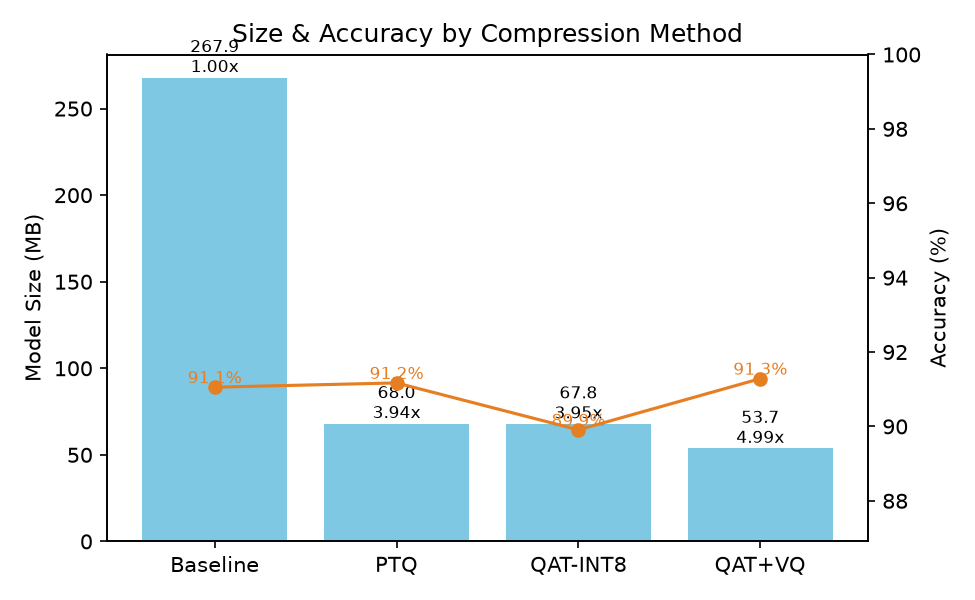
\includegraphics[width=0.75\textwidth]{figures/distilbert_size_acc.png}
\caption{DistilBERT / SST-2: model size and accuracy by compression
method. QAT+VQ is simultaneously the smallest and most accurate.}
\label{fig:distilbert}
\end{figure}

\subsection{GPT-2 / WikiText-2: A Genuine Pareto Point}

\begin{table}[h]
\centering
\begin{tabular}{lccc}
\toprule
Model & Perplexity & Size (MB) & Compression \\
\midrule
Baseline    & 25.85 & 497.8 & 1.00$\times$ \\
PTQ         & 25.87 & 125.3 & 3.97$\times$ \\
QAT-INT8    & 25.11 & 125.3 & 3.97$\times$ \\
GPTQ        & 25.86 & 125.3 & 3.97$\times$ \\
AWQ         & 25.87 & 125.5 & 3.97$\times$ \\
QAT+VQ (ours) & 26.12 & 96.8 & 5.14$\times$ \\
\bottomrule
\end{tabular}
\caption{GPT-2 (124M) / WikiText-2 test perplexity. Unlike the
classification result, QAT+VQ does not beat PTQ outright here; it is
23\% smaller for a $\sim$1\% relative perplexity increase.}
\label{tab:gpt2wt2}
\end{table}

On a generative task (Table~\ref{tab:gpt2wt2}), QAT+VQ does not dominate
PTQ, GPTQ, or AWQ on perplexity, forming instead a Pareto point: 23\%
smaller than any of the INT8-only methods for a roughly 1\% relative
perplexity cost. We report this honestly as a trade-off rather than
overstating it as a win --- the task-dependence of whether the hybrid
wins outright (classification) or trades off (generation) is itself a
finding worth noting for practitioners choosing a compression strategy.

\begin{figure}[h]
\centering
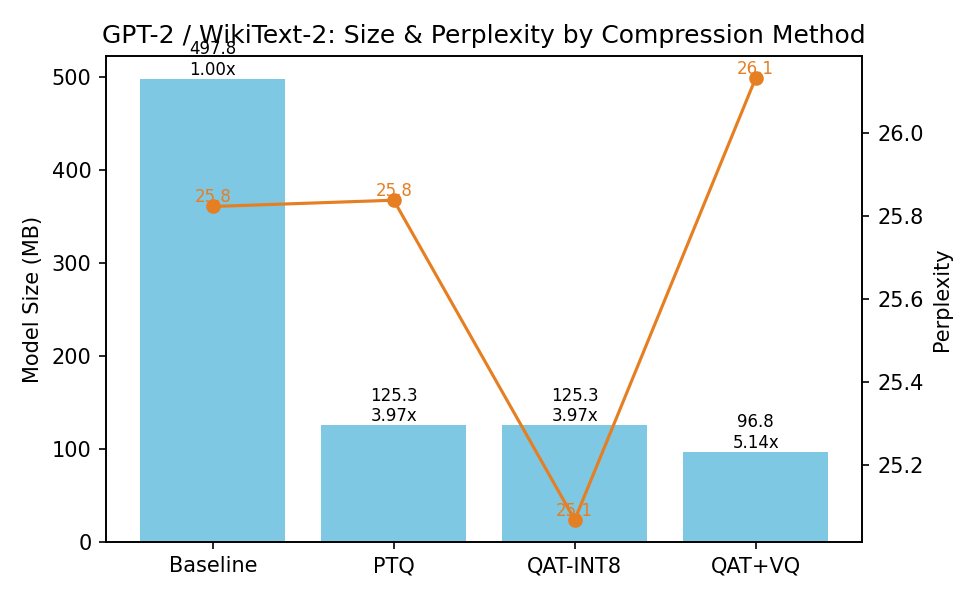
\includegraphics[width=0.75\textwidth]{figures/gpt2wt2_size_ppl.png}
\caption{GPT-2 (124M) / WikiText-2: model size and perplexity by
compression method. QAT+VQ trades a small perplexity increase for the
smallest footprint of any method.}
\label{fig:gpt2wt2}
\end{figure}

\subsection{Scaling Study: 124M vs. 355M vs. 774M}
\label{sec:scaling}

To test whether the QAT+VQ trade-off improves or worsens as models scale,
we repeat the identical pipeline on GPT-2 at three sizes, holding the
dataset, calibration subset size (20M characters), and method fixed.

\begin{table}[h]
\centering
\begin{tabular}{lcccc}
\toprule
Scale & Method & Perplexity & Size (MB) & Compression \\
\midrule
124M & Baseline / PTQ / QAT-INT8 / QAT+VQ & 24.33 / 24.35 / 24.14 / 24.76 & 497.8 / 125.3 / 125.3 / 96.8 & --- / 3.97$\times$ / 3.97$\times$ / 5.14$\times$ \\
355M & Baseline / PTQ / QAT-INT8 / QAT+VQ & 18.40 / 18.41 / 18.34 / 18.65 & 1419.4 / 356.7 / 356.7 / 255.6 & --- / 3.98$\times$ / 3.98$\times$ / 5.55$\times$ \\
774M & Baseline / PTQ / QAT-INT8 / QAT+VQ & 16.22 / 16.22 / 16.88 / 16.64 & 3096.3 / 777.3 / 777.3 / 540.5 & --- / 3.98$\times$ / 3.98$\times$ / 5.73$\times$ \\
\bottomrule
\end{tabular}
\caption{Scaling study across GPT-2 model sizes on matched WikiText-103
calibration data (20M characters at every scale). All four methods are
complete at every scale with no remaining data confounds.}
\label{tab:scaling}
\end{table}

\begin{figure}[h]
\centering

\includegraphics[width=\textwidth]{figures/scaling_comparison.png}
\caption{Size (left) and relative perplexity cost versus baseline
(right) by compression method, across all three GPT-2 scales. The
compression trend (left) is monotonic; the quality-cost trend (right) is
not.}
\label{fig:scaling}
\end{figure}

Two trends emerge, and they diverge (Figure~\ref{fig:scaling}):

\textbf{Compression improves monotonically with scale.} QAT+VQ's
compression ratio rises from 5.14$\times$ at 124M to 5.55$\times$ at 355M
to 5.73$\times$ at 774M. Larger models have more parameter redundancy for
product quantization to exploit, and the fixed, small codebook overhead
matters proportionally less as the compressed matrices grow.

\textbf{The perplexity gap versus PTQ does not shrink monotonically.} It
narrows from +1.68\% at 124M to +1.30\% at 355M, then widens sharply to
+2.59\% at 774M --- ending worse than the smallest model's starting gap.
A simpler two-point study (124M, 355M only) would have suggested a clean
``everything improves with scale'' narrative; the third point reveals a
more nuanced picture, which we report as-is rather than omitting the
inconvenient data point.

A related, arguably more surprising finding: \textbf{the simple INT8-only
QAT baseline, with no vector quantization at all, shows the same
scale-dependent reversal.} It outperforms the uncompressed baseline by
0.8\% and 0.3\% at 124M and 355M respectively, then underperforms it by
4.1\% at 774M. This was independently confirmed on matched calibration
data (ruling out a data-budget artifact as the explanation) and suggests
that scale-dependent quantization sensitivity at this model-size range is
not unique to vector quantization --- a finding of independent interest
beyond the specific hybrid method proposed here.

We additionally observe that codebook fine-tuning's benefit shrinks with
scale: it improved the 355M model's perplexity by approximately 0.35,
but only by 0.01 at 774M (with the second of two fine-tuning epochs
actually regressing slightly, correctly discarded by a best-checkpoint
guard). Larger models' k-means-initialized codebooks appear to already be
close to as good as further gradient-based fine-tuning can achieve within
a comparable training budget.

\subsection{Qualitative Generation Check}

Perplexity is a proxy for output quality, not a direct measure of it. We
generated text from the 124M baseline and QAT+VQ models on four held-out
prompts using greedy decoding. Both models produce fluent, topically
coherent continuations consistent with their Wikipedia-derived training
data. The most visible difference is that the QAT+VQ model shows a
somewhat higher tendency toward short repetition loops (e.g., restating a
clause verbatim) on two of four prompts, while the baseline does not
exhibit this in the same examples. Content coherence and topical relevance
are otherwise comparable. This is consistent with, and gives qualitative
texture to, the small but real perplexity gap reported in
Table~\ref{tab:gpt2wt2} --- the quality cost of compression manifests
primarily as increased repetition rather than incoherent output.

\section{Limitations}

This study is restricted to encoder-only classification (DistilBERT) and
decoder-only generation (GPT-2) up to 774M parameters; it does not test
billion-plus-parameter models where GPTQ and AWQ's advantages are most
pronounced in the literature, nor architectures such as Mixture-of-Experts
or non-Transformer designs. WikiText and SST-2 are single-domain,
single-language benchmarks. The 774M scaling point, while fully resolved on
matched calibration data, was computed across two separate Kaggle sessions
(due to session-length limits) using a checkpoint-recovery procedure rather
than a single uninterrupted run; while we verified this does not change the
final result, it is a departure from the other two scale points'
single-session execution. The qualitative generation check used a small,
fixed set of four prompts with greedy decoding only; a larger-scale human
evaluation would be needed to draw stronger conclusions about output
quality beyond the illustrative comparison presented here.

\section{Conclusion}

We presented a corrected hybrid of quantization-aware training and vector
quantization for transformer compression, diagnosed the specific design
choices (codebook size, weight-space versus activation-space application)
that caused a naive version of this idea to underperform simple baselines,
and evaluated the fix rigorously against literature-standard methods
across two task types and three model scales. The method outright wins on
classification and forms an honest, disclosed Pareto trade-off on
generation; its compression advantage provably improves with scale, while
its quality cost does not follow a simple monotonic pattern --- a finding
we consider more useful, precisely because it resists a tidy narrative,
than a cleaner-looking two-point result would have been.

\section*{Reproducibility}

Code, trained checkpoints' generation scripts, full experiment logs, and
per-experiment result files are publicly available at
\url{https://github.com/abdurrahmanrussel/QAT-VQ-Compression}, organized
as one branch per experiment (\texttt{distilbert-sst2-qatvq},
\texttt{gpt2-wikitext2-qatvq}, \texttt{gpt2medium-wikitext103-qatvq}),
each with a detailed \texttt{RESULTS.md} documenting exact commands,
hyperparameters, and — where relevant — the debugging process itself.

\bibliographystyle{plainnat}
\bibliography{references}

\end{document}
